\section{The game concept}

After the exploration of the game concepts presented before, the ideas for three
games were constructed. These games have been named 'Territory Takeover', 'The
War Game' and 'The Mine Game', for descriptive purposes.\newline 

The three games have all been initially proposed for development within a common
framework, but after close evaluation of the time and effort implications, the
decision was made to develop only one of them as proof-of-concept, while keeping
the others as proposals for future work.\newline

The game that has been chosen for this project is the one defined as 'The War
Game'. It promisses to be the game to offer a panoptic multiplayer experience,
both as a semi-core and casual game, while filling a gap in the current offer of
gaming experience by exploring the concept of Location-based Real Time Strategy
games. \newline

The purpose of this project is to create a Real Time Tactics game that can be
played outdoors and focus on social interaction through augmenting reality. It
should be fast paced, while not demanding on time and game or technical skills.
An important subject of focus is strategy as a catalyst for social
bonding.\newline

As a byproduct of the requirements mentioned, an element of focus is to make the
game appealing a wide spectrum of population. It is to provide casual gameplay
that can also be taken to more serious levels, according to the skill of the
players themselves.\newline

The main goal is to develop the game and provide appealing functionality and
dynamics. The second goal is to test whether a broad spectrum of population may
enjoy this game and if not. \newline


\begin{figure}
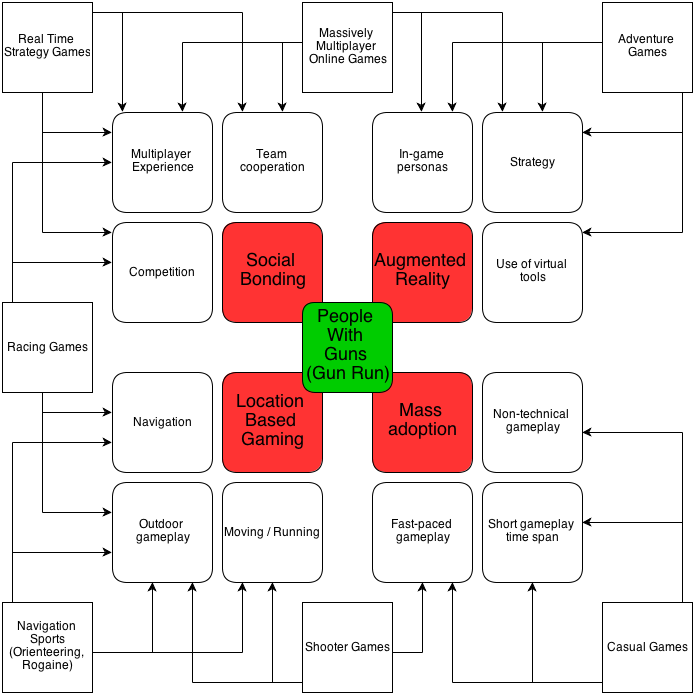
\includegraphics[height=6in,width=6in]{./images/diagrams/ConstructionOfPeopleWithGuns.png}
\caption{\small \sl Conceptual construction of ''People With Guns''(''Gun Run'') 
\label{fig:concept_construction}}
\end{figure}



\subsection{The War Game}

The 'War Game', which has later been named 'People With Guns', is a GPS-based
game in which two teams fight a last-man-standing battle. Each person gets to
choose between a number of character types in the game. How fast one moves in
the game equals how fast one runs in real life.\newline

The player can choose between four types of characters : Medic, Sniper, Scout,
Marine - each with their own specific weapons and health, fitting different
roles within the game.\newline

The rules of the game are simple: two times fight a virtual battle. One team's
purpose is to defeat the opposite team with the means given: each player's real
life movement and the virtual weapons and powerups for fighting. The interface
with the so-called 'weapons' and 'powerups' is layed out in the form of buttons
that are shown on the bottom of the screen. Each weapon or powerup has the
following attributes: range, cooldown, duration, damage. By default weapons have
instant effect(therefore no duration) and powerups have no damage(but they have
a duration) - the only exception is the 'Heal' ability. Both weapons and
cooldowns have a range - an area of effect for their use. If a target falls
within that area, the weapon or powerup of choice can be used. After the
activation of a weapon or powerup, it will be availavbe for use after a time
given by its 'cooldown' attribute. In the case of powerups('Invisibility' and
'Shield'), their time span during which they are in effect after activation will
be given by the 'duration' attribute. \newline

The players are to perform complex communication between each other verbally,
thus maintaining social contact as long as they are in each other's proximity.
For the case of players that are too far away from the rest of their team, a
number of preset messages are provided for quickly exchanging information
between them(such as asking for help, cover or for healing) without distracting
them from the gameplay.\newline

The purpose of this game is to add to the experience of a group of people,
without taking too much focus upon itself. Social bonding and team building are
the goal to be achieved through strategy, tactics and a fun, light game to bring
it all together.\newline

While sliding away from the idea of enhancing a tour mobile app, it was observed
that there are no location-based Real Time Strategy games in existence, or at
least not visible to the thorough search performed to find any.\newline

Based on the previous ideas and some concepts provided into a few games or game
ideas such as Warfinger GPS, MobileWar and racing and navigation games, three
game ideas have been crystalized.\newline 

The games proposed for this project have been :
\begin{enumerate}	
	\item \textbf{Territory Takeover}
	\item \textbf{The War Game}
	\item \textbf{The Mine Game}
\end{enumerate}

1. The \textbf{Territory Takeover} game is a multiplayer, team versus team
competitive game. The players or game author define an area of play, which will
be automatically divided into multiple areas defined by a grid. Each division
will be marked by a 'flag' (a GPS marker). To capture the area division, a team
must capture its flag. The game ends when all flags have been captured and the
winner is the team with most captured flags. Each flag may be given a time that
a player must spend next to it in order to capture it. Once a flag (and
implicitly the territory) is captured, it remains so until the end of the game.
The winner can be decided on flag counting or, alternatively, each flag may
receive a number of points, according to the size of the territory marked by it
and the difficulty of the terrain. \newline

This game can be enhanced with the use of virtual tools or weapons. For the
purpose of this project, the following tools/weapons have been considered :
\begin{enumerate}
	
	\item The \textbf{blocker} is an ability that can be used by each player to
	block an opponent from moving. The 'attacker' 'activates' the ability and a
	circle around him is drawn to show the range in which he can shoot. If an
	opponent enters the range area, the 'attacker' will select him on the map and
	shoot. The 'victim' will receive a notification that he is immobilized. A
	circle or rectangle will be defined around him and he will not be allowed to
	move outside of it for a given time, say 30 seconds or 1 minute. If he does, he
	gets disqualified and kicked out of the game. An alternate solution would be
	that the team loses points, for the case that this is the scoring methodology
	implemented.
	 
	\item \textbf{unblocker} is an ability that an immobilized player can use.
	For this project, it will only work on the person that uses the ability. The
	effect is that a person that is immobilized gets the waiting time halved.
	
\end{enumerate}
Both the abilities have a common cooldown timer. That means that if a player
immobilizes somebody and is immediately immoblized himself, he won't be able to
use the unblocker because of the cooldown following the usage of the
blocker.\newline

For time and effort reasons, this game will not be implemented now, but kept as
future work: it can be added as an extra game type within the app in
development.\newline

2. \textbf{The War Game} is inspired by Real Time Strategy and Shooter games.
Two teams are formed. The area of play may be limited or unlimited. Each
player can choose between a number of characters. The first proposal has been
for four character types: Defender, Marine, Sniper and Heavy Trooper. Each of
the four characters has special abilities and characteristics :
\begin{enumerate}
	
	\item The \textbf{Defender} has the ability to generate shields for short
	periods of time. Members of the team can hide behind those shields for defence.
	The Defender may also act as a Medic and heal or revive members of the team. He
	has low health, long ability cooldowns and a sidearm with short range, small
	damage and fast cooldowns .
	
	\item The \textbf{Marine} has a weapon that can shoot a medium range with
	medium damage and fast cooldowns. He has medium health. 
	
	\item The \textbf{Sniper} has two weapons : the sniper rifle that can shoot at
	distant ranges and deal large damage to single targets and the sidearm, which
	is the same as the Defender's. His health is low, just like the Defender's. The
	sniper shot may penetrate the Defender's shield and cause reduced damage to one
	target.	
	
	\item The \textbf{Heavy Trooper} has three weapons : the bazooka, the sidearm
	and mines. The bazooka is a mid-range weapon with splash damage - it therefore
	can be fired against compact groups, such as the ones that might be hiding
	behind a shield. The bazooka cannot deal damage through the shield, but it may
	be shot next to it, causing damage from the side. The damage to each target
	varies from moderate to small, depending how far they are from the center of
	the 'projectile explosion'. The mines can be placed randomly on the map and
	their 'explosions' will not affect the members of the Heavy Trooper's team.
	Also they cannot be triggered by the members of his team. The damage dealt will
	be moderate, with splash damage, just like the bazooka projectile. The bazooka
	and the mines have long cooldowns, therefore the sidearm is added. The Heavy
	Trooper has high health.
	 
\end{enumerate}


3. \textbf{The Mine Game} is inspired by the classical game Minesweeper,
Warfinger GPS and running games such as the ones in Tourality. It is essentially
a single player game that can be played by many for score ranking. It may be
adapted in various ways directly into the 'War Game'. The purpose of the game is
that the player uses his phone as a mine detector and defuser and navigates
through a virtual mine field, racing against time to get from a start point to
an end point. A variant of this game could be of a team helping a designated
player navigate through the mine field without touching any mines.\newline

Some advantages and drawbacks can be highlighted for these games:\newline

\textbf{Advantages}: They don't require specialized gear and setting, nor
do they need long amounts of time to be played. They can be enjoyed with a
bunch of friends on a sunny weekend afternoon.\newline
\textbf{Drawbacks}: They highly depend on GPS accuracy. This issue may
affect gameplay. This applies especially to the 'Mine Game', which would need
pinpoint accuracy most of the time. \newline

The similarity of the construction of the three above-mentioned games would
allow us to use a common framework that will enable multiplayer interaction for
both 'free for all'/'skirmish' and 'team versus team' approaches and permit the
implementation of the 'Mine Game' along with the others. They would require a
server to centralize player information such as GPS data and various attributes.
Because the games proposed are fast-paced, they require quick response times
from the server, client and and the use of a fast and reliable protocol between
them.\newline

The games are proposed with group teambuilding and recreation in mind. They
require team strategy and cooperation. Territory Takeover allows for both team
versus team and free for all gameplay, allowing for both small and large groups
to play. The War Game is to be a fast paced game spanning a time interval in the
range of a few tens of minutes. Although it contains some Shooter elements -
such as the act of shooting itself - it focuses on strategy and tactics. Quick
reflexes might be required to shoot, but not to aim Where it lacks the realism
of simulations or the immersion of classical computer Real Time Strategy games,
it gains in the intensity of real-life experience and teamwork, without requiring
specialized equipment or highly developed skills. Therefore, the game that is
about to be developed fills a niche between casual and immersive games, bringing
focus to social interaction.\newline

From these three games, the one that was chosen for implementation was 'The War
Game', because it offers a more versatile gameplay, conceptually permitting
a larger number of players, while imposing less time and space restrictions.


\subsubsection{Implementation}

Implementation will mean developing a server and a client application from
scratch, covering all the functionality needed for the main game - the so-called
'War Game' to work according to its description.

\subsubsection{Schedule}
This project, consisting of one server and one client application, was planned
to be developed in four steps:


\begin{enumerate}
  \item \textbf{Development} - During the first iteration of development, the
  most basic features of the game are to be implemented: basic server
  functionality that would allow the game to work, basic client functionality
  and the 'War Game' without all features.(2 months)
  
  \item \textbf{Testing and Evaluation} - During this phase, the game and its
  functionality will be livetested for feasibility and quality. New ideas will
  be sought and documented. Most importantly, player feedback will be
  gathered.(1 month)
  
  \item \textbf{Development} - During the second iteration of development, the
  'War Game' will be completed and, using its framework, the 'Territory
  Takeover' game will be implemented. Bugs will be removed and tweaks will be
  made to the framework and the game concepts to match the player feedback.(2
  months)
  
  \item \textbf{Evaluation and Completion} - During the second evaluation phase,
  both games will be tested for playability, player feedback will be gathered
  and the Dissertation Paper will be completed.(1 month)
    
\end{enumerate}



\subsection{Gameplay}

The gameplay will be presented as a typical scenario of interacting with the
application:

\begin{enumerate}
  \item First of all, in order to get in the game, the player must connect to
  the server. Because this version of the game was created for testing purposes
  only, the server can only host one game. Once there is somebody playing,
  nobody else can join the game. A few seconds after everyone has left the game
  (gone back to the Main Menu), the server will reset itself and accept clients
  once more.
  
  \item Second, once the player has connected to the server, he will be
  presented with the Game Lobby. This is where he joins a team, sets his
  nickname and chooses his character type.

  \item Third, after the player has finished setting up, he can mark himself as
  'Ready' to play the game. If all the players are Ready, the server will send a
  five second countdown and send the signal to enter the game - at which point,
  all connected clients will switch to the game screen and the players can
  start playing.
  
  \item Once in the game, the player's weapons will be enabled only when the
  teams satisfy the starting condition - for now, that means that the average
  positions of all the members of the two teams must be at least 150m apart and
  the members of each team must be at most 20m away from the center position of
  their team.
 
\end{enumerate}

The strategy of the teams can vary and will be more succesful when they devise
one in which they help and back each other, by complementing their skills. That
is why this game can provide both easy, fun gameplay and serious and complicated
strategies, based on the intention of the people playing. Different combinations
of players in each team, according to the needs and style of each player are
possible - and they lead to ever-different approaches in the game.\newline

The game ends when one of the teams is eliminated. Each player's 'character' or
'profession' has a number of associated health points. When the number of health
points reaches zero, the player is eliminated from the game and shown a dialog
giving the options to either quit the game or spectate.\newline

